\documentclass[a5paper,12pt,fleqn,titlepage,twoside]{book}
\usepackage{rotating}
\usepackage{setspace}
\onehalfspacing
\usepackage{url}
\usepackage[utf8]{inputenc}
\usepackage[ngerman]{babel}
\usepackage{amsfonts}
\usepackage[T1]{fontenc}
\usepackage{makeidx}
\usepackage{multicol}
\usepackage{rotating}
\usepackage{subfigure}
\usepackage{xcolor}
\usepackage{graphicx}% or \usepackage[pdftex]{graphicx}
\usepackage[dvips]{hyperref}

\hypersetup{%
pdfauthor={Michael Durrer},pdftitle={Gegen den Strom - Eine Seele packt aus},
   pdfstartview={Fit},
   pdfkeywords={sdl,c++},
colorlinks={true},linkcolor={blue},filecolor={magenta},pagecolor={red},urlcolor={cyan},citecolor={green}
}
\author{Michael Durrer}
\date{2007-01-24}
\title{Gegen den Strom}
\begin{document}
\begin{titlepage}

\begin{center}

\begin{LARGE}\textbf{Gegen den Strom}\end{LARGE}
\newline
\newline
\newline
\begin{small}Written with \LaTeX in \emph{Kile} by Michael Durrer\newline\end{small}
\newline
\newline
\newline
\emph{Letzte \"Anderung am \today.}

\end{center}

\end{titlepage}
 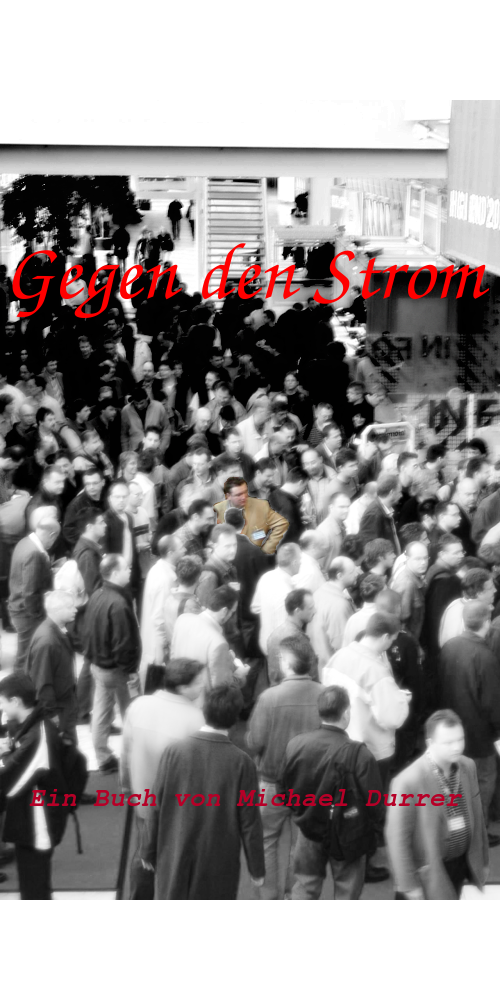
\includegraphics{cover.png}\hfill\vfill
\newpage
\tableofcontents
\part{Beweggründe}
\label{part:Beweggründe}
Es gab viele Gründe für mich, dieses Buch zu schreiben, doch einige waren besonders anregend hierfür. Auf solche Anregungen möchte ich in diesem Teil des Buches eingehen.

\chapter{Wieso man ein Buch schreibt}
\section{Meine Wenigkeit}
Zuerst möchte ich ein wenig etwas über meine Wenigkeit schreiben. Nicht aus egomanen Gründen, nein, sondern weil ich dem Leser einen Eindruck über den Autor vermitteln möchte, dem er hier für die nächsten Stunden und Tage seines Lebens seine Zeit widmen wird mit dem Konsum dieses Buches. Halten sich mich für regressiv, aber gerade in der heutigen Zeit halte ich es für wichtiger denn je, solche Gesten zu schätzen und vorallem zu erhalten	.

Schliesslich empfinde ich das als eine grosse Ehre, wenn jemand sich soviel zeit für meine Werke nimmt, es redet ja schon kaum jemand so lange mit mir... kaum zu glauben, nicht? Es sei ihnen verziehen, so mag ich ja auch nicht immer auf andere Kommunikations- und Sozialpartner den Eindruck eines gepflegten oder intellektuell angehauchten Mitbürgers machen.


\end{document}
